\documentclass{article}
\usepackage[margin=1in]{geometry}
\usepackage{amsmath}
\usepackage{amssymb}
\usepackage{amsthm}
\usepackage{bm}
\usepackage{hyperref}
\usepackage{graphicx}
\usepackage{caption}
\usepackage{listings}
\usepackage{xcolor}
\usepackage{float}
\usepackage{placeins}
\graphicspath{{figures/}}

% Code style
\lstdefinestyle{code}{
  basicstyle=\ttfamily\small,
  numbers=left,
  numberstyle=\tiny,
  numbersep=8pt,
  keywordstyle=\color{blue},
  commentstyle=\color{teal!70!black},
  stringstyle=\color{orange!70!black},
  showstringspaces=false,
  breaklines=true,
  frame=single,
  framerule=0.3pt,
  rulecolor=\color{black!15}
}
\lstset{style=code}

\title{Optimization and Regularization Techniques in Practice}
\author{}
\date{\today}

\begin{document}
\maketitle
\tableofcontents
\FloatBarrier

\section{Adaptive Optimizers: Adam, RMSprop, and Beyond}
Gradient-based optimization adapts learning rates to the geometry of the loss surface. Adaptive optimizers rescale parameter-specific learning rates using running statistics of the gradients, enabling faster convergence on ill-conditioned objectives.

\subsection{RMSprop}
RMSprop maintains an exponential moving average of squared gradients:
\begin{align}
  \mathbf{v}_t &= \rho \mathbf{v}_{t-1} + (1-\rho) \nabla_{\boldsymbol{\theta}} \mathcal{L}_t \odot \nabla_{\boldsymbol{\theta}} \mathcal{L}_t, \\
  \boldsymbol{\theta}_{t+1} &= \boldsymbol{\theta}_t - \eta \frac{\nabla_{\boldsymbol{\theta}} \mathcal{L}_t}{\sqrt{\mathbf{v}_t + \epsilon}},
\end{align}
with decay $\rho \approx 0.9$ and numerical stabilizer $\epsilon \approx 10^{-8}$. The adaptive denominator dampens updates along directions with persistent large gradients.

\subsection{Adam and AdamW}
Adam augments RMSprop with momentum by tracking both first and second moments:
\begin{align}
  \mathbf{m}_t &= \beta_1 \mathbf{m}_{t-1} + (1-\beta_1) \nabla_{\boldsymbol{\theta}} \mathcal{L}_t, \\
  \mathbf{v}_t &= \beta_2 \mathbf{v}_{t-1} + (1-\beta_2) \nabla_{\boldsymbol{\theta}} \mathcal{L}_t \odot \nabla_{\boldsymbol{\theta}} \mathcal{L}_t.
\end{align}
Bias correction compensates for the initialization at zero:
\begin{align}
  \hat{\mathbf{m}}_t &= \frac{\mathbf{m}_t}{1-\beta_1^{t}}, &
  \hat{\mathbf{v}}_t &= \frac{\mathbf{v}_t}{1-\beta_2^{t}}.
\end{align}
The parameter update becomes
\begin{equation}
  \boldsymbol{\theta}_{t+1} = \boldsymbol{\theta}_t - \eta \frac{\hat{\mathbf{m}}_t}{\sqrt{\hat{\mathbf{v}}_t} + \epsilon}.
\end{equation}
AdamW decouples weight decay from the adaptive gradient by applying L2 regularization separately:
\begin{equation}
  \boldsymbol{\theta}_{t+1} = (1-\eta \lambda)\boldsymbol{\theta}_t - \eta \frac{\hat{\mathbf{m}}_t}{\sqrt{\hat{\mathbf{v}}_t} + \epsilon},
\end{equation}
where $\lambda$ is the weight decay coefficient. Decoupling preserves the intended magnitude control while retaining Adam's adaptive step.

\subsection{AdaBelief, AdaFactor, and Yogi}
Modern variants tweak moment tracking for stability in large-scale training.
\begin{itemize}
  \item \textbf{AdaBelief} replaces squared gradients with the squared deviation from the first moment, reducing variance in stationary regions.
  \item \textbf{AdaFactor} factorizes the second-moment matrix into row and column statistics, dramatically lowering memory footprint for transformers.
  \item \textbf{Yogi} adds a signed adjustment to the second moment, preventing $\mathbf{v}_t$ from growing unbounded and stabilizing training on sparse gradients.
\end{itemize}

\begin{figure}[H]
  \centering
  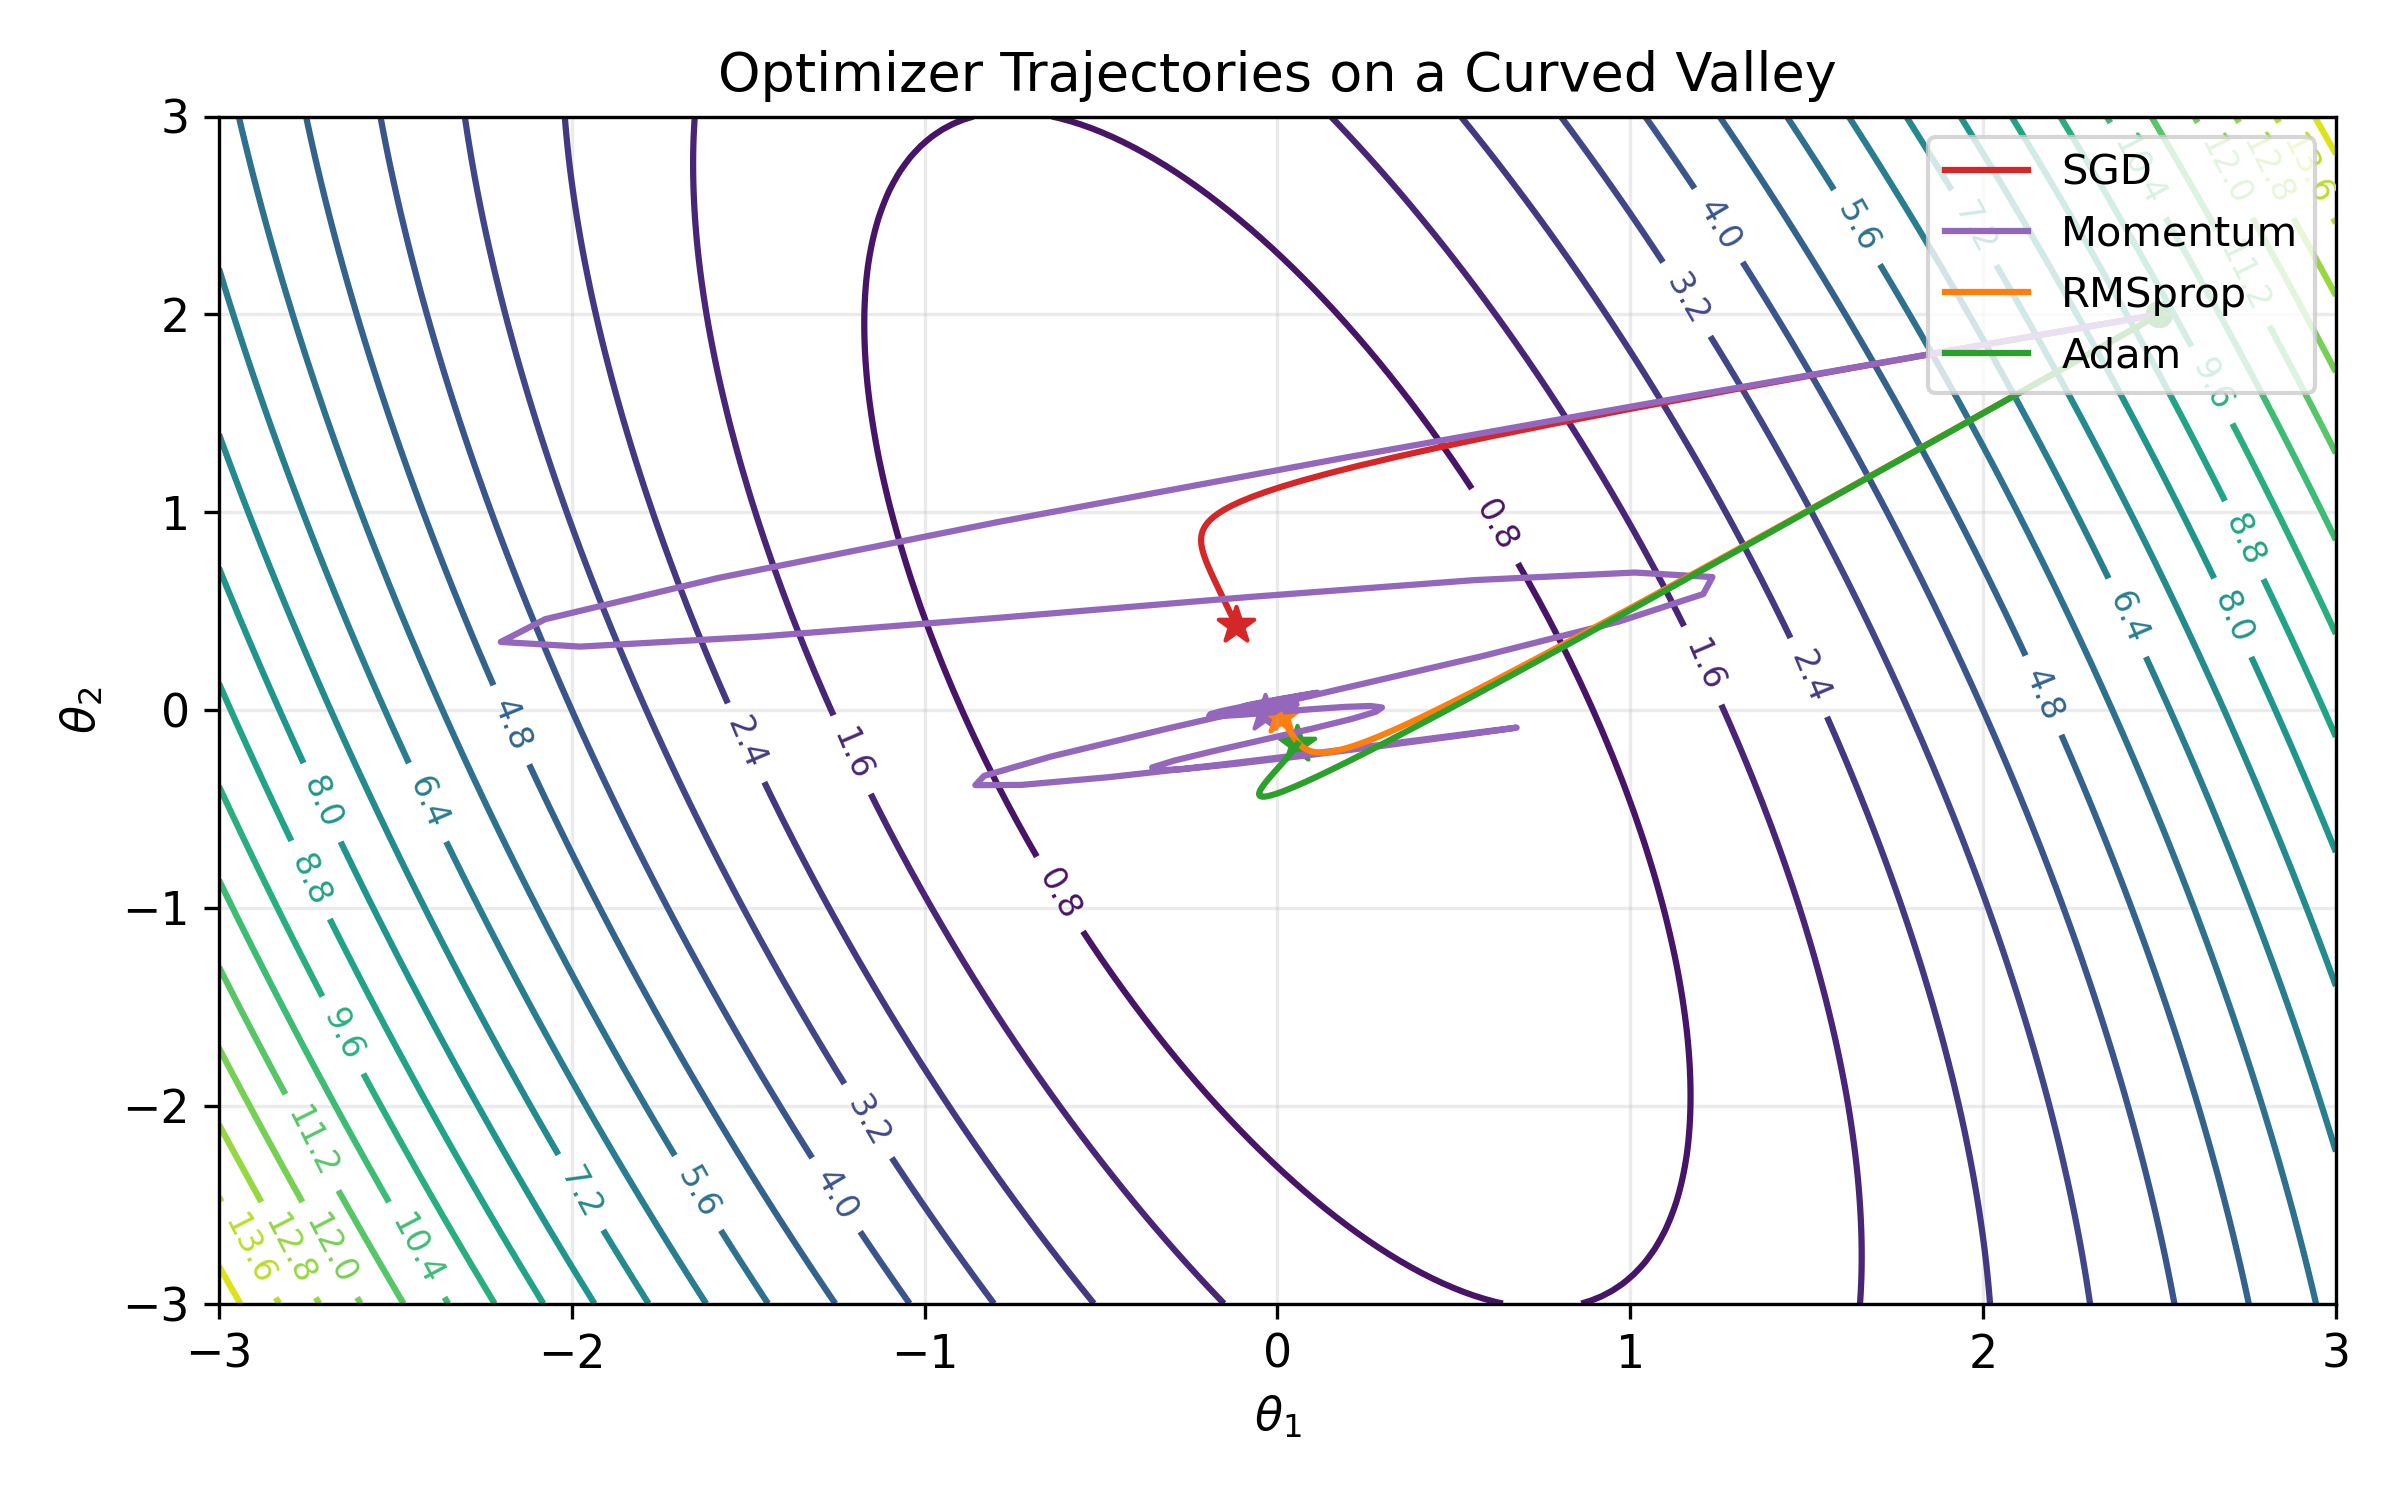
\includegraphics[width=0.8\textwidth]{optimizer_dynamics.png}
  \caption{Optimization trajectories on a valley-shaped loss for SGD, momentum, RMSprop, and Adam. Adaptive methods align steps with narrow curvature directions.}
  \label{fig:optimizer_dynamics}
\end{figure}
\FloatBarrier

\subsection{Implementation Considerations}
Large-scale training stacks multiple tricks: gradient clipping, mixed precision, and decoupled weight decay. The following snippet shows an AdamW optimizer with gradient clipping and cosine annealing:

\begin{lstlisting}[language=Python, caption={AdamW with gradient clipping and cosine learning rate schedule.}]
import torch
from torch.nn.utils import clip_grad_norm_
from torch.optim.lr_scheduler import CosineAnnealingLR

optimizer = torch.optim.AdamW(model.parameters(), lr=3e-4,
                              betas=(0.9, 0.999), eps=1e-8, weight_decay=0.01)
scheduler = CosineAnnealingLR(optimizer, T_max=1000, eta_min=1e-5)

for step, batch in enumerate(dataloader, start=1):
    loss = compute_loss(model, batch)
    loss.backward()
    clip_grad_norm_(model.parameters(), max_norm=1.0)
    optimizer.step()
    scheduler.step()
    optimizer.zero_grad()
\end{lstlisting}

\section{Batch Normalization and Layer Normalization}
Normalization stabilizes the distribution of activations, reducing covariate shift between layers and accelerating convergence.

\subsection{Batch Normalization}
Given a mini-batch $\mathcal{B} = \{\mathbf{h}_i\}_{i=1}^{m}$, BatchNorm normalizes each feature dimension:
\begin{align}
  \boldsymbol{\mu}_\mathcal{B} &= \frac{1}{m} \sum_{i=1}^{m} \mathbf{h}_i, &
  \boldsymbol{\sigma}_\mathcal{B}^2 &= \frac{1}{m} \sum_{i=1}^{m} (\mathbf{h}_i - \boldsymbol{\mu}_\mathcal{B})^{\odot 2}, \\
  \hat{\mathbf{h}}_i &= \frac{\mathbf{h}_i - \boldsymbol{\mu}_\mathcal{B}}{\sqrt{\boldsymbol{\sigma}_\mathcal{B}^2 + \epsilon}}, &
  \mathbf{y}_i &= \boldsymbol{\gamma} \odot \hat{\mathbf{h}}_i + \boldsymbol{\beta}.
\end{align}
Running averages of $\boldsymbol{\mu}_\mathcal{B}$ and $\boldsymbol{\sigma}_\mathcal{B}^2$ provide consistent statistics during inference. BN implicitly regularizes by injecting noise from batch sampling, improving generalization but complicating recurrent models and tiny-batch regimes.

\subsection{Layer Normalization}
LayerNorm operates across features within a single example, avoiding dependence on batch size. For activations $\mathbf{h}$ of dimension $d$,
\begin{equation}
  \mu = \frac{1}{d} \sum_{j=1}^{d} h_j, \quad \sigma^2 = \frac{1}{d} \sum_{j=1}^{d} (h_j - \mu)^2, \quad \hat{h}_j = \frac{h_j - \mu}{\sqrt{\sigma^2 + \epsilon}}.
\end{equation}
A shared pair of learnable parameters $(\gamma, \beta)$ rescales and recenters the normalized output. LN excels in transformer architectures and autoregressive models where batch statistics vary greatly.

\subsection{Comparative Analysis}
\begin{itemize}
  \item \textbf{Sensitivity to batch size:} BN degrades when batch statistics are noisy; LN remains stable.
  \item \textbf{Regularization effect:} BN's stochasticity acts as implicit regularization, often reducing the need for dropout.
  \item \textbf{Computation:} BN requires synchronizing statistics across devices for data-parallel training, whereas LN is embarrassingly parallel but adds per-sample overhead.
\end{itemize}

\begin{figure}[H]
  \centering
  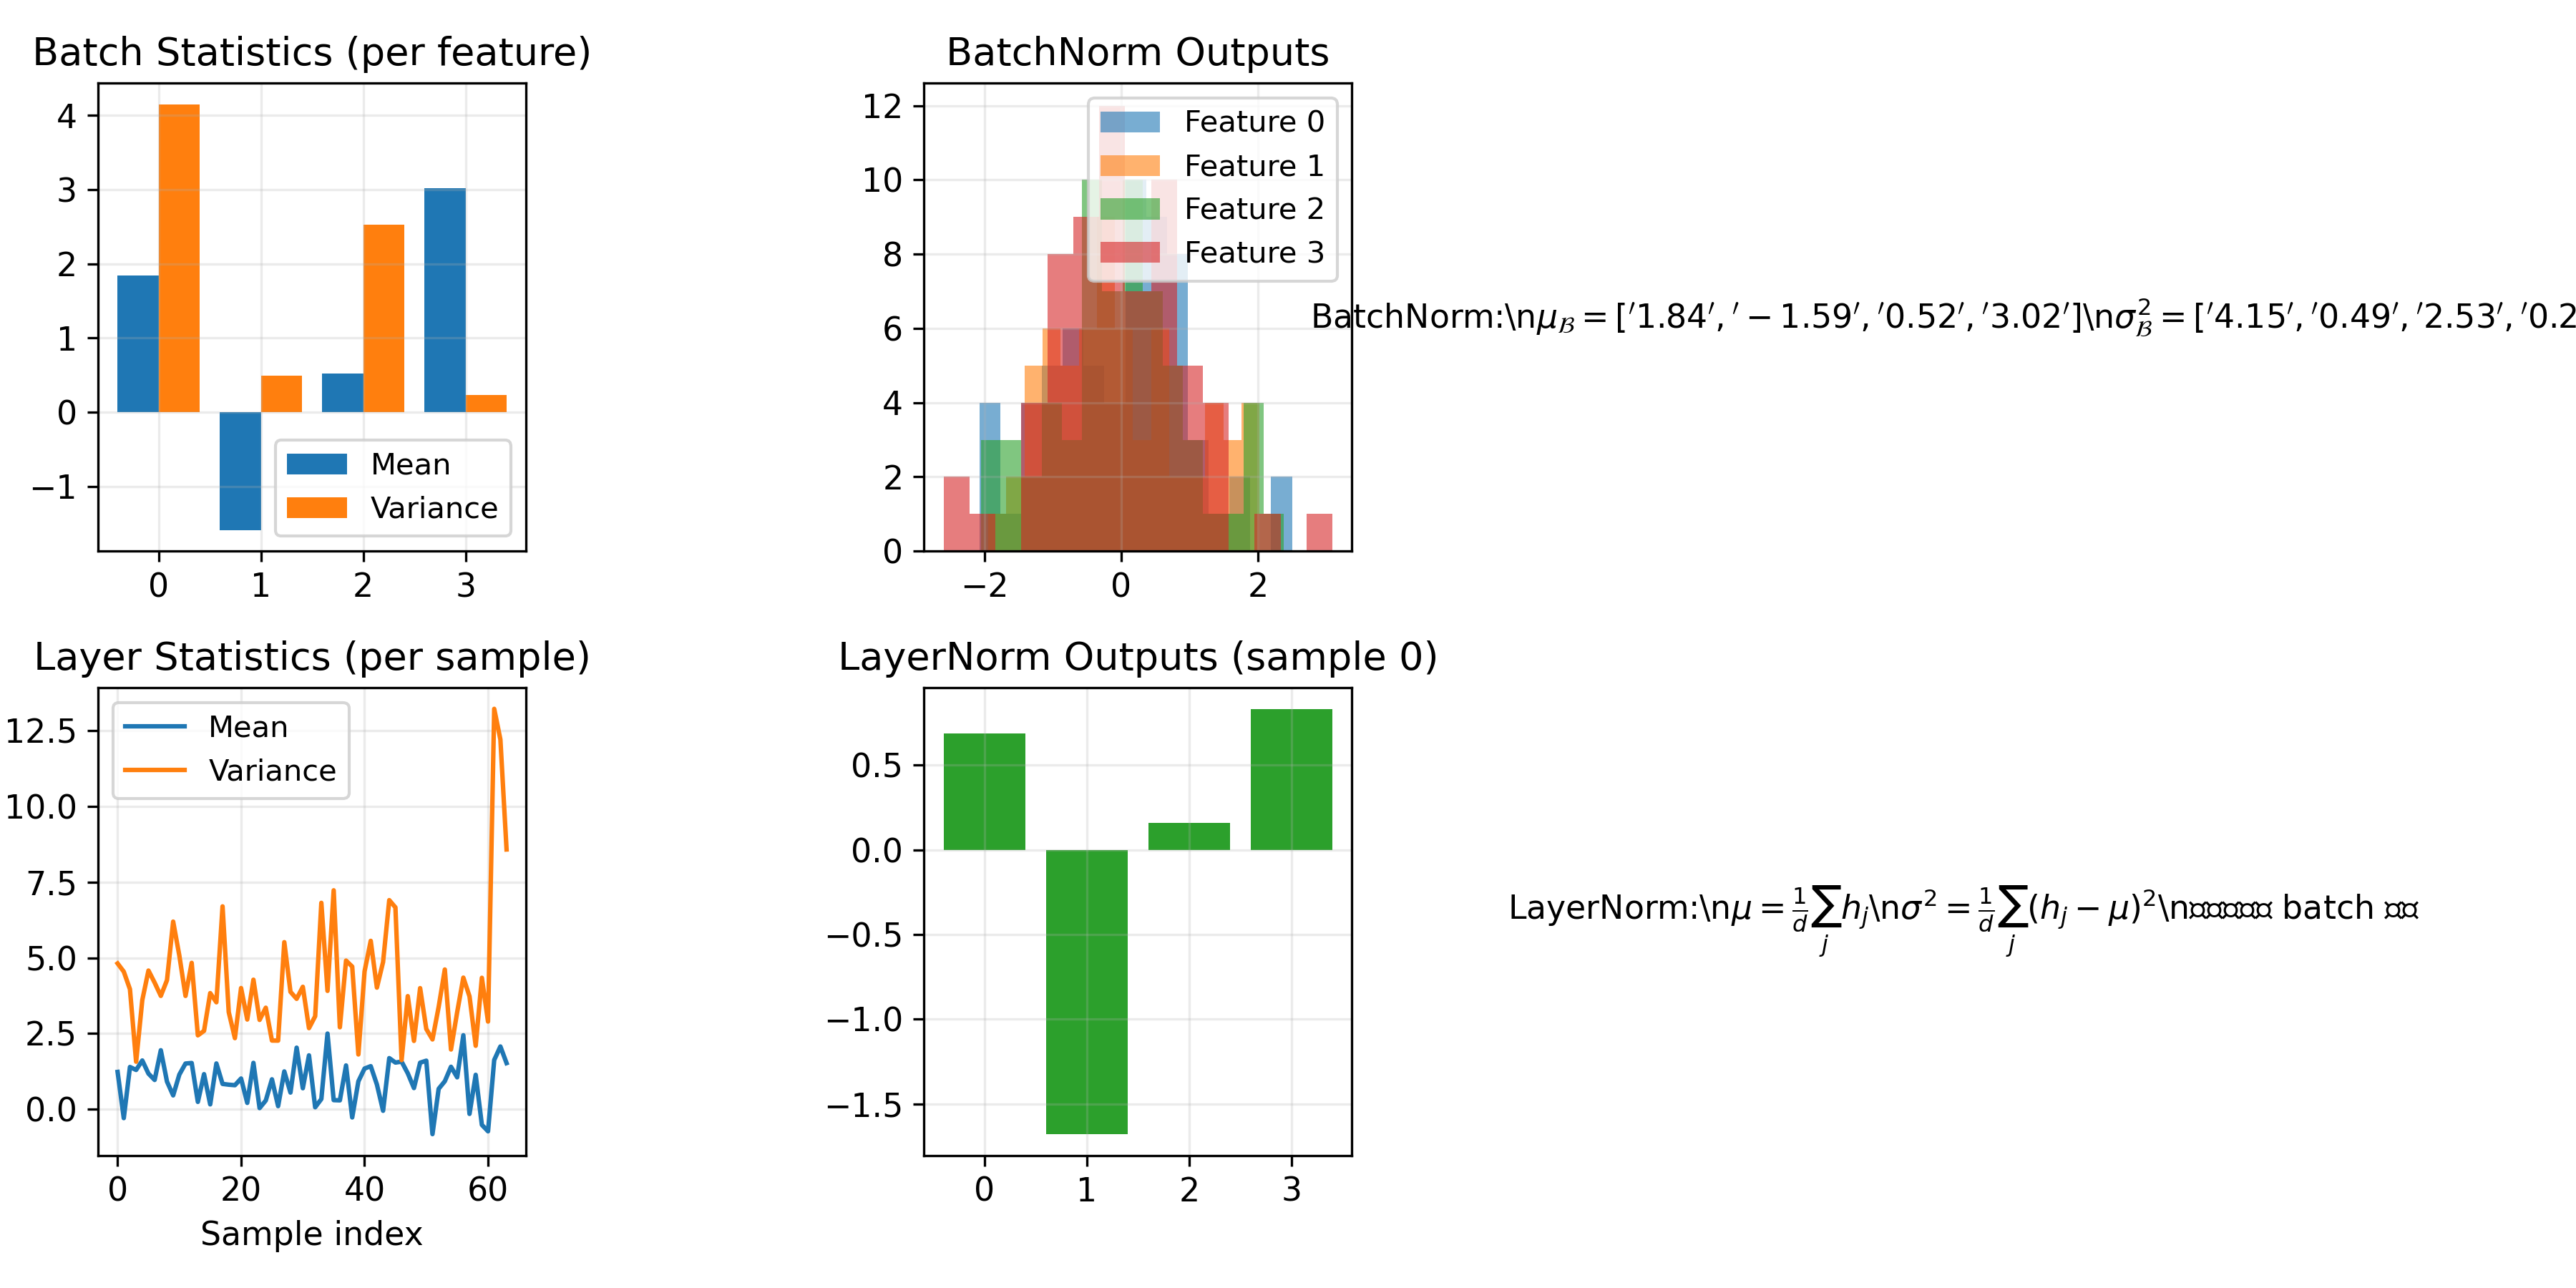
\includegraphics[width=0.8\textwidth]{normalization_comparison.png}
  \caption{Distribution shift before and after BatchNorm and LayerNorm. BN uses batch-wide statistics, while LN normalizes each token independently.}
  \label{fig:normalization_comparison}
\end{figure}
\FloatBarrier

\section{Learning Rate Scheduling and Warm-up}
Learning rate schedules balance fast initial progress with stable convergence. Warm-up mitigates the mismatch between randomly initialized parameters and adaptive optimizers that rely on accumulated statistics.

\subsection{Step, Exponential, and Polynomial Decay}
Step decay multiplies $\eta_t$ by $\gamma < 1$ every $k$ epochs:
\begin{equation}
  \eta_t = \eta_0 \gamma^{\left\lfloor \frac{t}{k} \right\rfloor}.
\end{equation}
Exponential decay adjusts the rate continuously:
\begin{equation}
  \eta_t = \eta_0 \exp(-\lambda t).
\end{equation}
Polynomial decay interpolates between $\eta_0$ and $\eta_{\mathrm{end}}$ over $T$ steps:
\begin{equation}
  \eta_t = \eta_{\mathrm{end}} + (\eta_0 - \eta_{\mathrm{end}}) \left(1 - \frac{t}{T}\right)^{p}.
\end{equation}

\subsection{Cosine Annealing and Cyclical Policies}
Cosine annealing smoothly decays the learning rate to $\eta_{\min}$:
\begin{equation}
  \eta_t = \eta_{\min} + \frac{1}{2} (\eta_0 - \eta_{\min}) \left(1 + \cos\frac{\pi t}{T}\right).
\end{equation}
Cyclical learning rates oscillate between bounds, promoting exploration of the loss landscape. For example, triangular schedules increase linearly to $\eta_{\max}$ and decay back to $\eta_{\min}$ within a cycle.

\subsection{Warm-up Strategies}
Warm-up ramps the learning rate from zero to the target value over $T_w$ steps:
\begin{equation}
  \eta_t =
  \begin{cases}
    \eta_{\mathrm{target}} \frac{t}{T_w}, & 0 \le t \le T_w, \\
    \text{Schedule}(t - T_w), & t > T_w.
  \end{cases}
\end{equation}
Transformers often employ linear warm-up followed by inverse square root decay, $\eta_t \propto t^{-1/2}$. Warm-up prevents adaptive optimizers from overreacting to initial gradient noise when moment estimates are unreliable.

\begin{figure}[H]
  \centering
  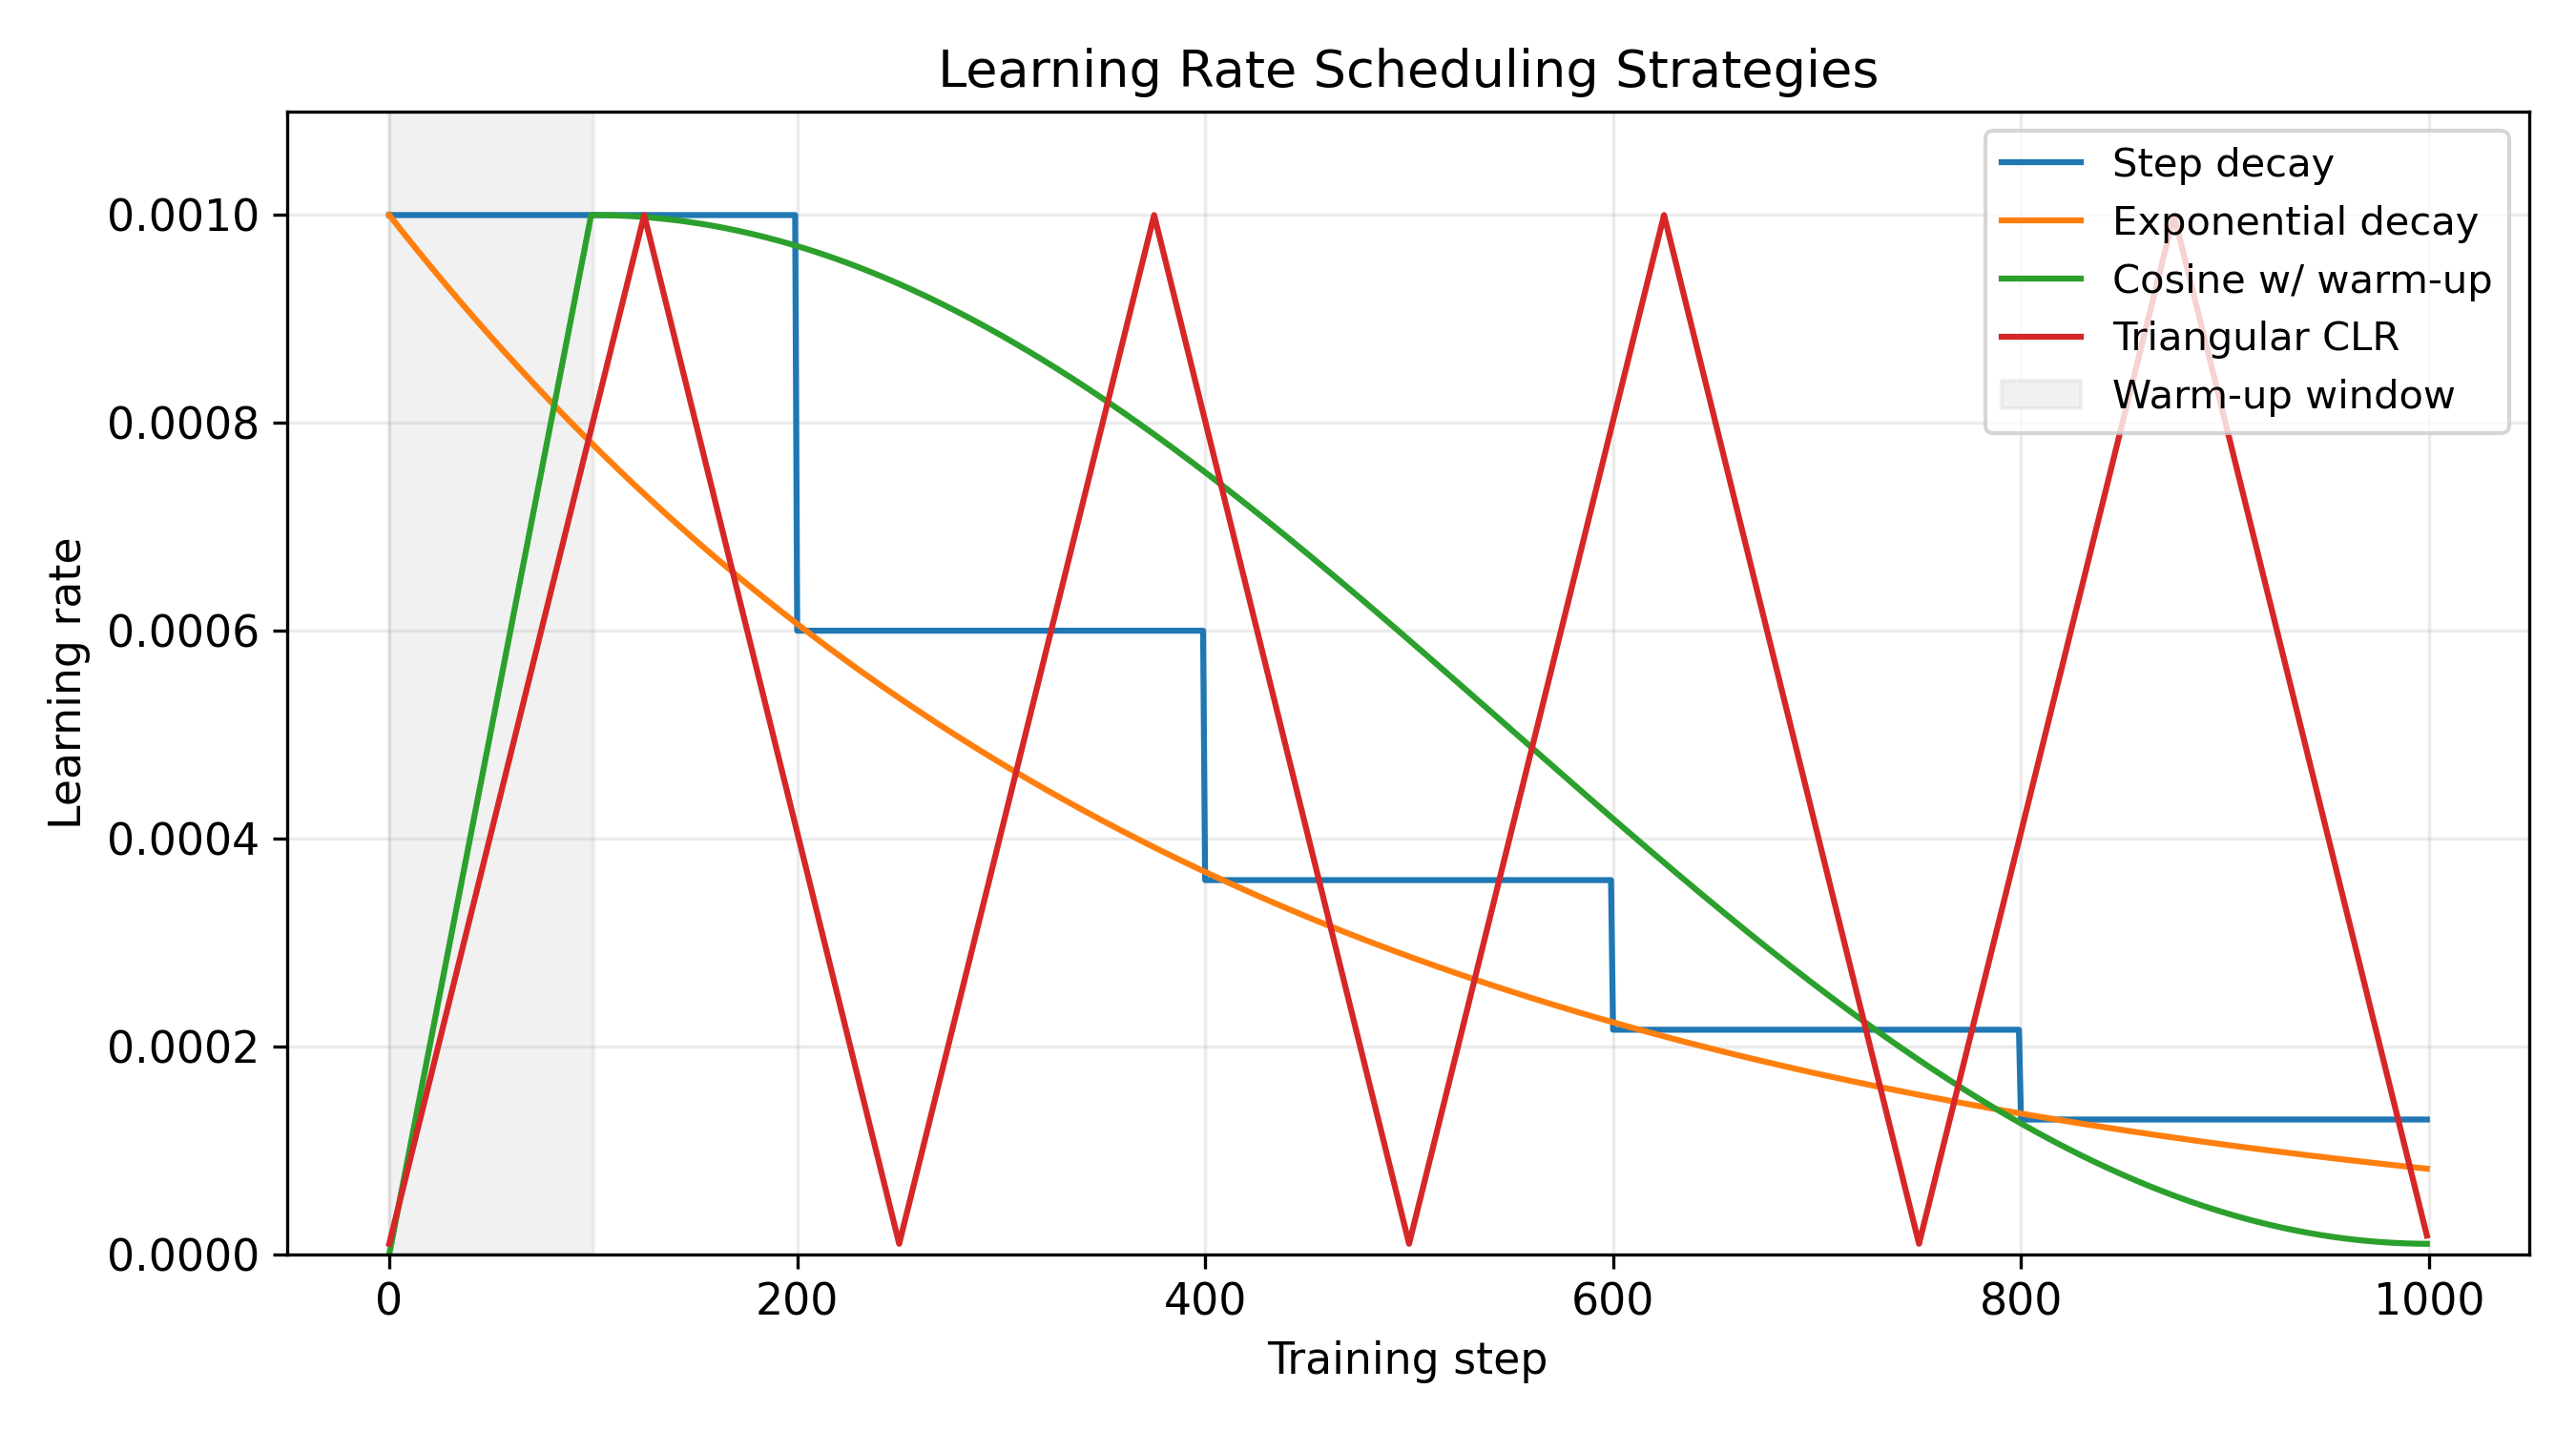
\includegraphics[width=0.85\textwidth]{learning_rate_policies.png}
  \caption{Comparison of step, cosine, cyclical, and warm-up learning rate policies. Warm-up smooths the start of training before the decay schedule begins.}
  \label{fig:learning_rate_policies}
\end{figure}
\FloatBarrier

\section{Data Augmentation and Transfer Learning}
Augmentation and transfer learning expand effective data coverage and reuse pretrained representations to accelerate convergence and boost performance on scarce datasets.

\subsection{Classical and Advanced Augmentations}
Spatial and photometric augmentations preserve labels while perturbing inputs:
\begin{itemize}
  \item \textbf{Geometric:} random crops, flips, rotations, and elastic deformations.
  \item \textbf{Photometric:} color jitter, histogram equalization, Cutout.
  \item \textbf{Mix-based:} Mixup forms convex combinations of pairs, $\tilde{\mathbf{x}} = \lambda \mathbf{x}_i + (1-\lambda)\mathbf{x}_j$, with targets $\tilde{\mathbf{y}} = \lambda \mathbf{y}_i + (1-\lambda)\mathbf{y}_j$.
  \item \textbf{Distributional:} RandAugment samples augmentation chains; AugMix blends multiple randomized augmentations with Jensen-Shannon consistency loss.
\end{itemize}

\subsection{Transfer Learning Workflow}
Transfer learning initializes a target model with pretrained weights $\boldsymbol{\theta}_{\mathrm{pre}}$ obtained on a source dataset $\mathcal{D}_{\mathrm{src}}$. Fine-tuning adapts the model to the target dataset $\mathcal{D}_{\mathrm{tgt}}$:
\begin{align}
  \boldsymbol{\theta}_0 &= \boldsymbol{\theta}_{\mathrm{pre}}, \\
  \boldsymbol{\theta}_{t+1} &= \boldsymbol{\theta}_t - \eta_t \nabla_{\boldsymbol{\theta}} \bigl[\mathcal{L}_{\mathrm{tgt}}(\boldsymbol{\theta}_t) + \lambda \mathcal{R}(\boldsymbol{\theta}_t - \boldsymbol{\theta}_{\mathrm{pre}})\bigr],
\end{align}
where $\mathcal{R}$ regularizes deviation from pretrained features (e.g., L2-SP, Fisher regularization). Layer-wise adaptive rate scaling (LARS/LAMB) can assign smaller learning rates to lower layers to preserve useful representations.

\subsection{Self-Supervised Pretraining}
Contrastive and masked-prediction objectives learn transferable features without labels. SimCLR maximizes agreement between augmented views via the NT-Xent loss:
\begin{equation}
  \mathcal{L}_{\mathrm{NT-Xent}} = -\sum_{i} \log \frac{\exp(\mathbf{z}_i \cdot \mathbf{z}_{i}' / \tau)}{\sum_{j} \mathbf{1}_{[j \neq i]} \exp(\mathbf{z}_i \cdot \mathbf{z}_j / \tau)}.
\end{equation}
Fine-tuning leverages these representations on downstream tasks with minimal labeled data.

\subsection{Practical Pipeline}
Figure~\ref{fig:augmentation_transfer_pipeline} summarizes a typical workflow that chains data augmentation, backbone pretraining, and task-specific heads.

\begin{figure}[H]
  \centering
  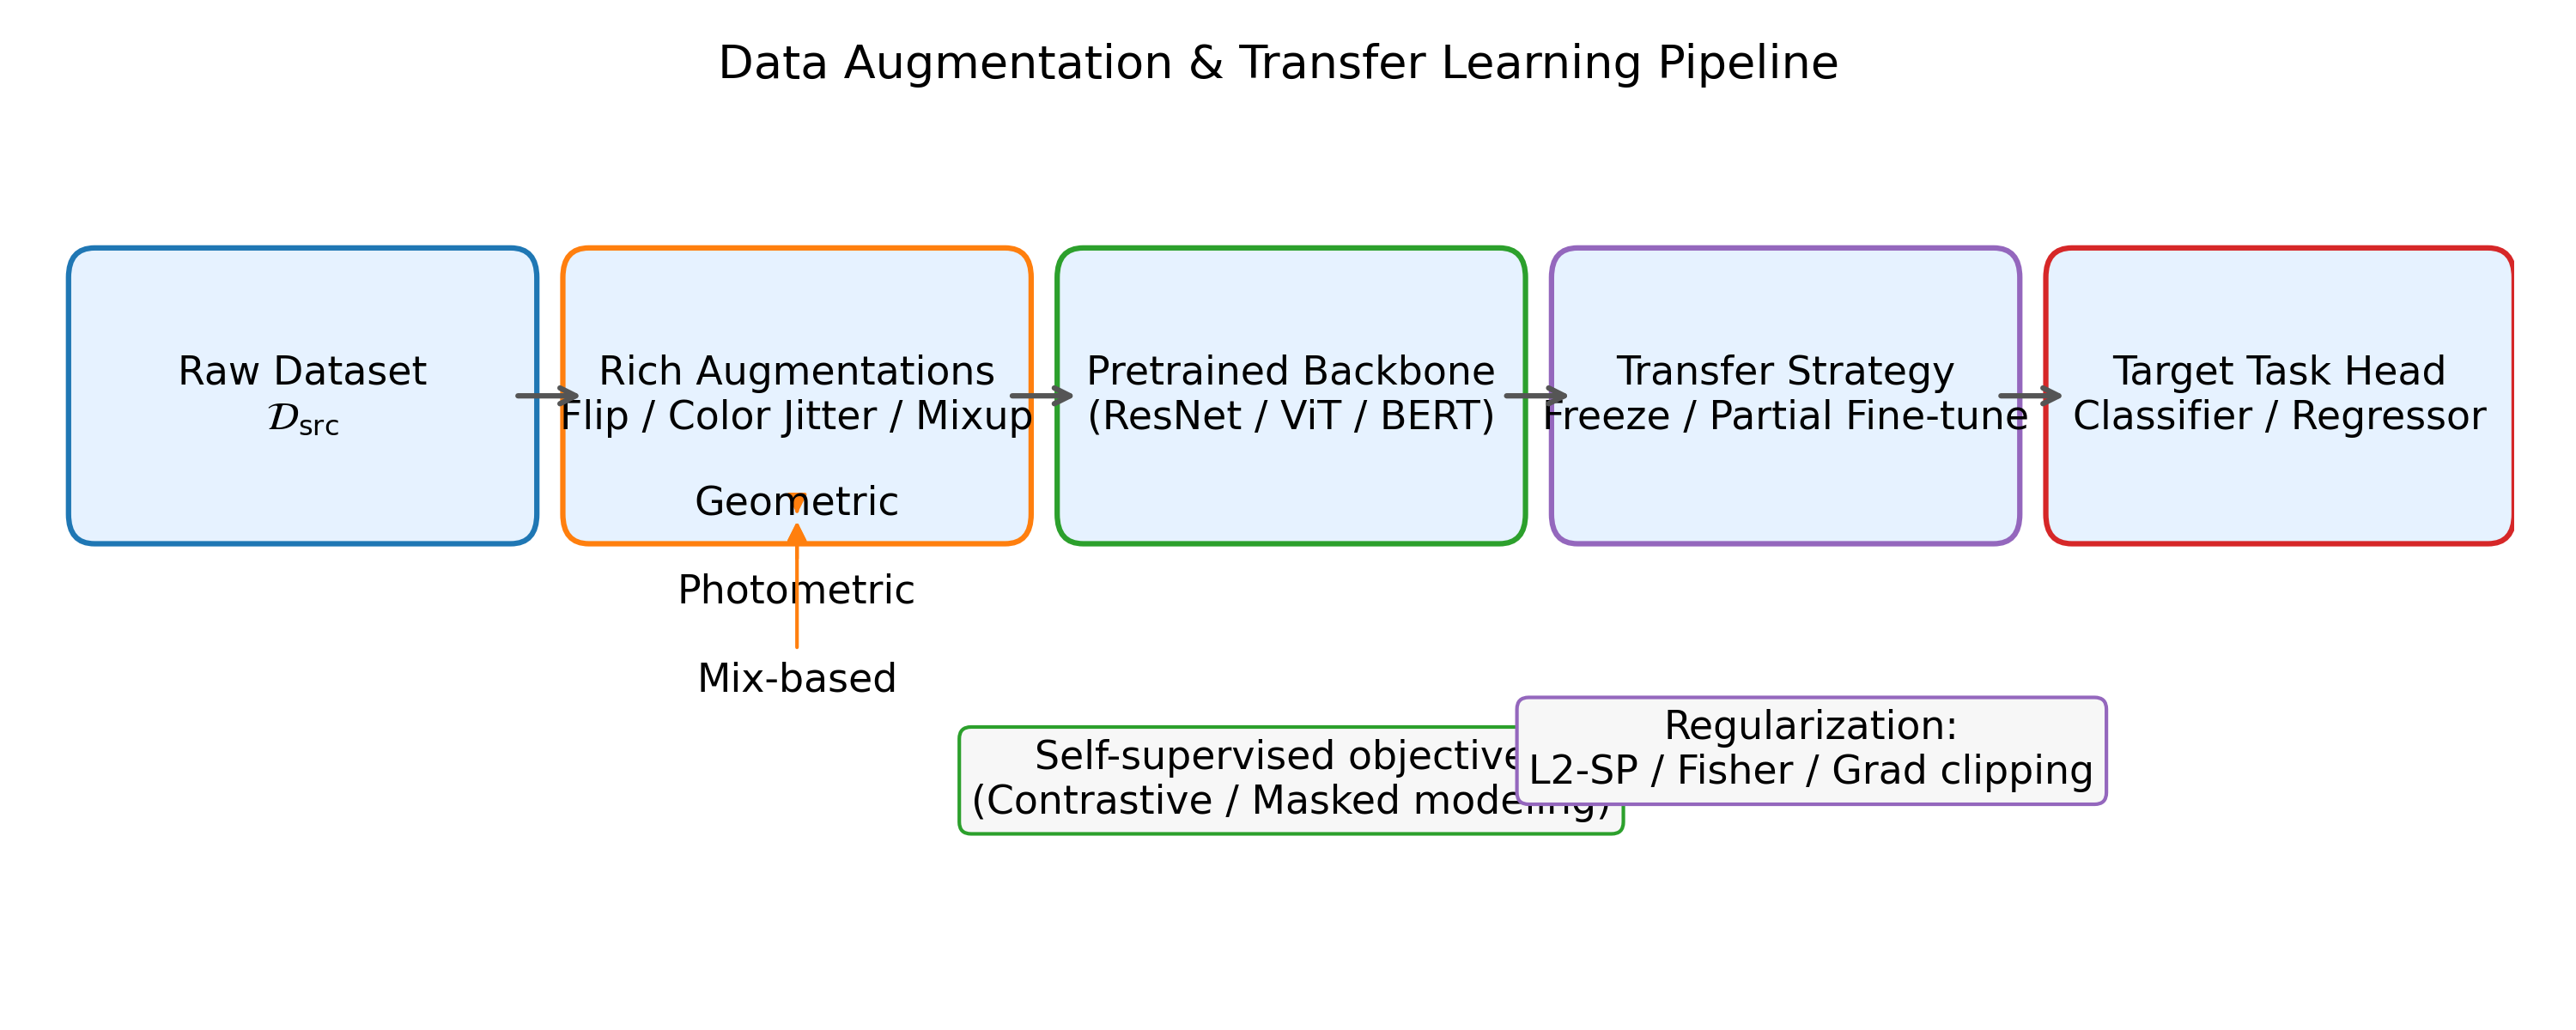
\includegraphics[width=0.9\textwidth]{augmentation_transfer_pipeline.png}
  \caption{Pipeline combining rich data augmentation with transfer learning. Augmented samples feed a pretrained backbone, optionally frozen, before adaptation on the target task.}
  \label{fig:augmentation_transfer_pipeline}
\end{figure}
\FloatBarrier

\section*{Further Reading}
\begin{itemize}
  \item Ilya Loshchilov and Frank Hutter. ``Decoupled Weight Decay Regularization.'' ICLR 2019.
  \item Sergey Ioffe and Christian Szegedy. ``Batch Normalization.'' ICML 2015.
  \item Leslie N. Smith. ``Cyclical Learning Rates for Training Neural Networks.'' WACV 2017.
  \item Tong He et al. ``Bag of Tricks for Image Classification with Convolutional Neural Networks.'' CVPR 2019.
\end{itemize}

\end{document}
